\chapter{System Overview}
\pagenumbering{arabic}

\GrG\ is a generative programming system for graph rewriting. \GrG\ is mainly designed for \emph{typed graphs}.  That means, graphs are not only nodes and edges, but labeled (\emph{attributed typed}) directed multigraphs. The type system is specified as class hierarchy, like classes in object oriented languages. Type systems for specific sets of graphs can be specified by user supplied graph meta models. Such a graph model describes a set of well-formed graphs, i.e.\ allowed node and edge types, their attributes and specific connection assertions. We'll build a graph model for a Turing machine in section \ref{anexample}.

\begin{figure}[htbp]
	\centering
  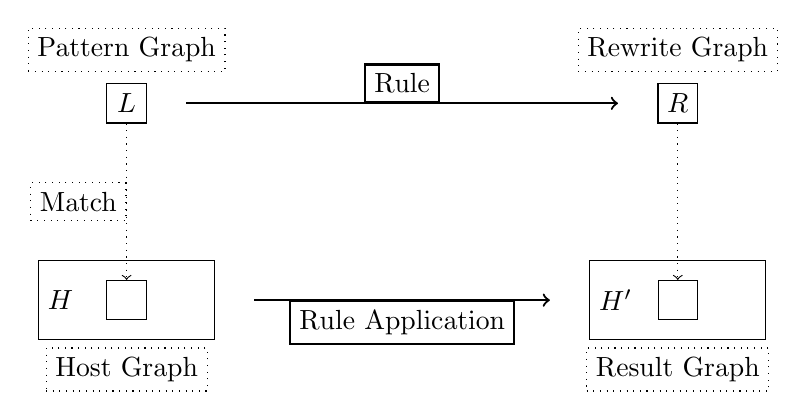
\begin{tikzpicture}
    \begin{scope}[minimum size=0.5cm]
      \tikzstyle{every node}=[draw]
      \node (L)     at (0   ,2.5) {$L$};
      \node (R)     at (7   ,2.5) {$R$};
      \node (mL)    at (0   ,0) {};
      \node (mR)    at (7   ,0) {};
      \node[text width=2cm,text badly ragged,minimum size=1cm] (H)     at (0   ,0) {$H$};
      \node[text width=2cm,text badly ragged,minimum size=1cm] (Hs)    at (7   ,0) {$H'$};
    \end{scope}

    \draw[dotted,->] (L) node[above=0.4cm] {Pattern Graph} -> (mL) node[left,midway]  {Match}   node[below=0.6cm] {Host Graph};
    \draw[dotted,->] (R) node[above=0.4cm] {Rewrite Graph} -> (mR)                              node[below=0.6cm] {Result Graph};

    \pgfsetshortenstart{0.5cm}
    \pgfsetshortenend{0.5cm}
    \draw[thick,->]  (L) -> (R)  node[above,midway] {Rule};
    \draw[thick,->]  (H) -> (Hs) node[below,midway] {Rule Application};
  \end{tikzpicture}
  \caption{Basic Idea of Graph Rewriting}
  \label{figrule}
\end{figure}

How does graph rewriting work? \GrG\ implements an SPO-based approach. Given a host graph $H$, each \emph{rewriting rule} $p: L \longrightarrow R$ consists of a pattern $L$ and a transformation specification $R$ in form of an adopted pattern graph. The process of rewriting searches a match $H_L \unlhd H$ (i.e.\ a graph homomorphism from $L$ to a subgraph of $H$) and rewrites $H_L$ to $R$. Nodes or edges added to $R$ (in compare to $L$) will be added $H_L$ and nodes or edges deleted in $R$ will be deleted in $H_L$. The homomorphism may not be unique.

We'll have a look at a small example. First we use a special case to construct our host graph: an empty pattern does always produce exactly one match (independently of the host graph). So starting with an empty host graph $H$ we construct an apple using
\[ p:  \begin{array}[c]{c} 
\includegraphics[width=3cm]{fig/empty} \end{array} \begin{array}[c]{c} \longrightarrow \end{array} \begin{array}[c]{c} 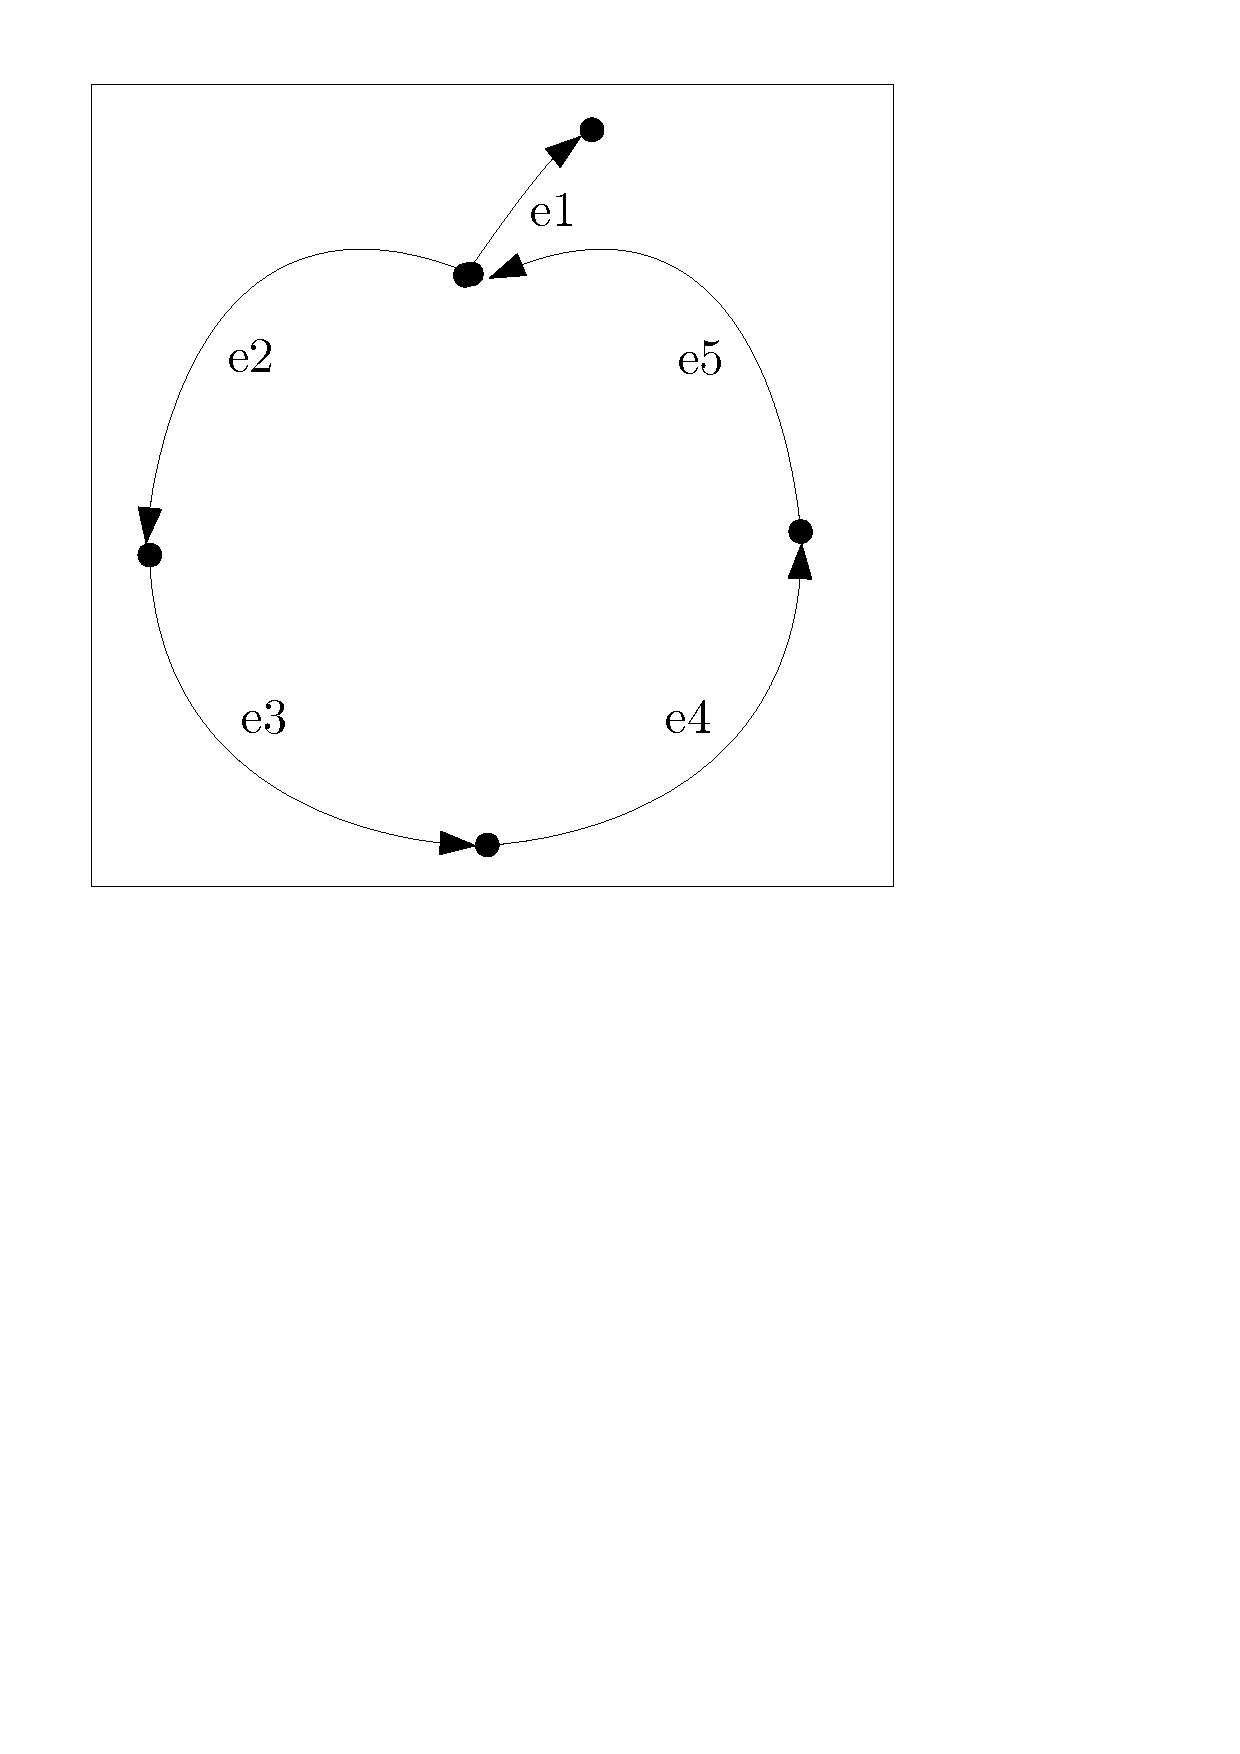
\includegraphics[width=3cm]{fig/apple} \end{array} \]
applied to $H$. We'll get the apple as new host graph $H'$. Now we want to rewrite our apple with stem to an apple with a leaflet. We use
\[ p':  \begin{array}[c]{c} 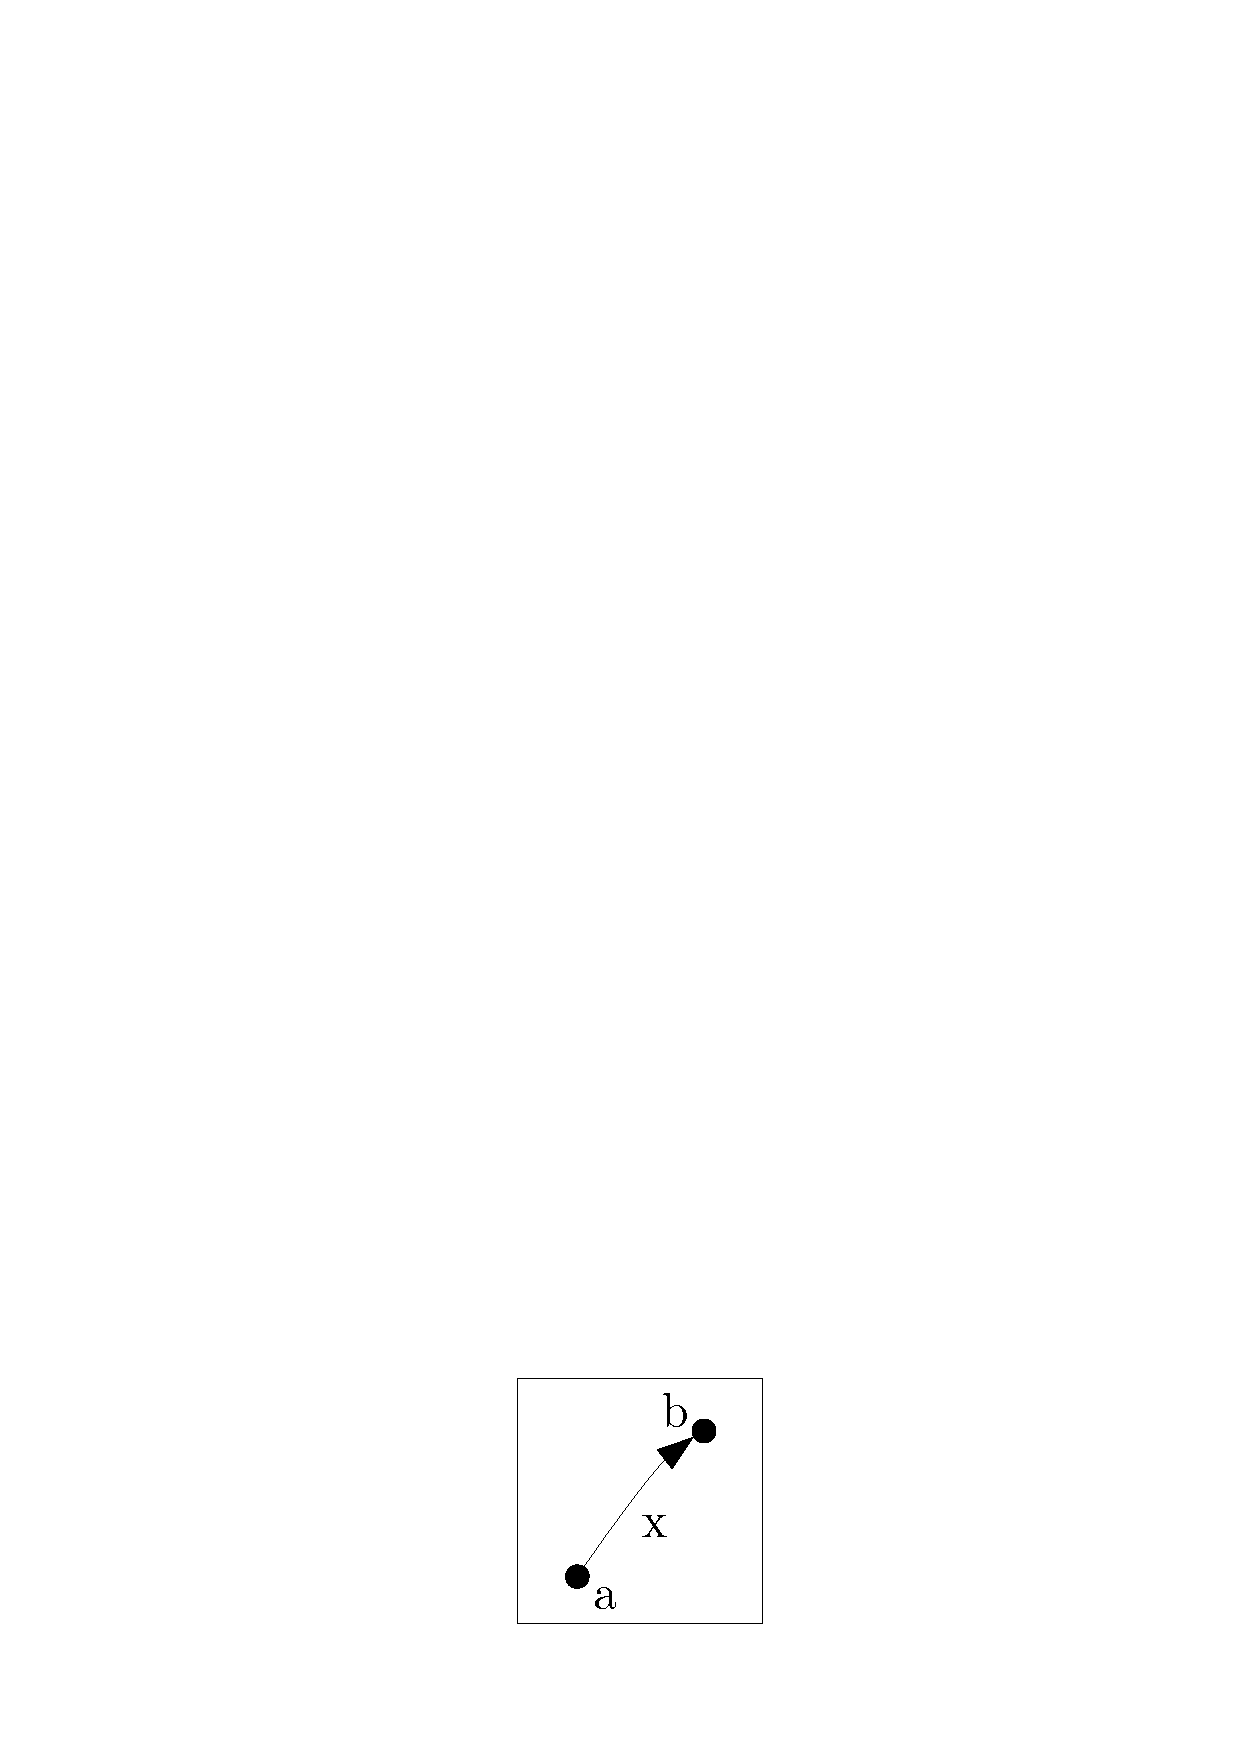
\includegraphics[height=1.25cm]{fig/stiel} \end{array} \begin{array}[c]{c} \longrightarrow \end{array} \begin{array}[c]{c} 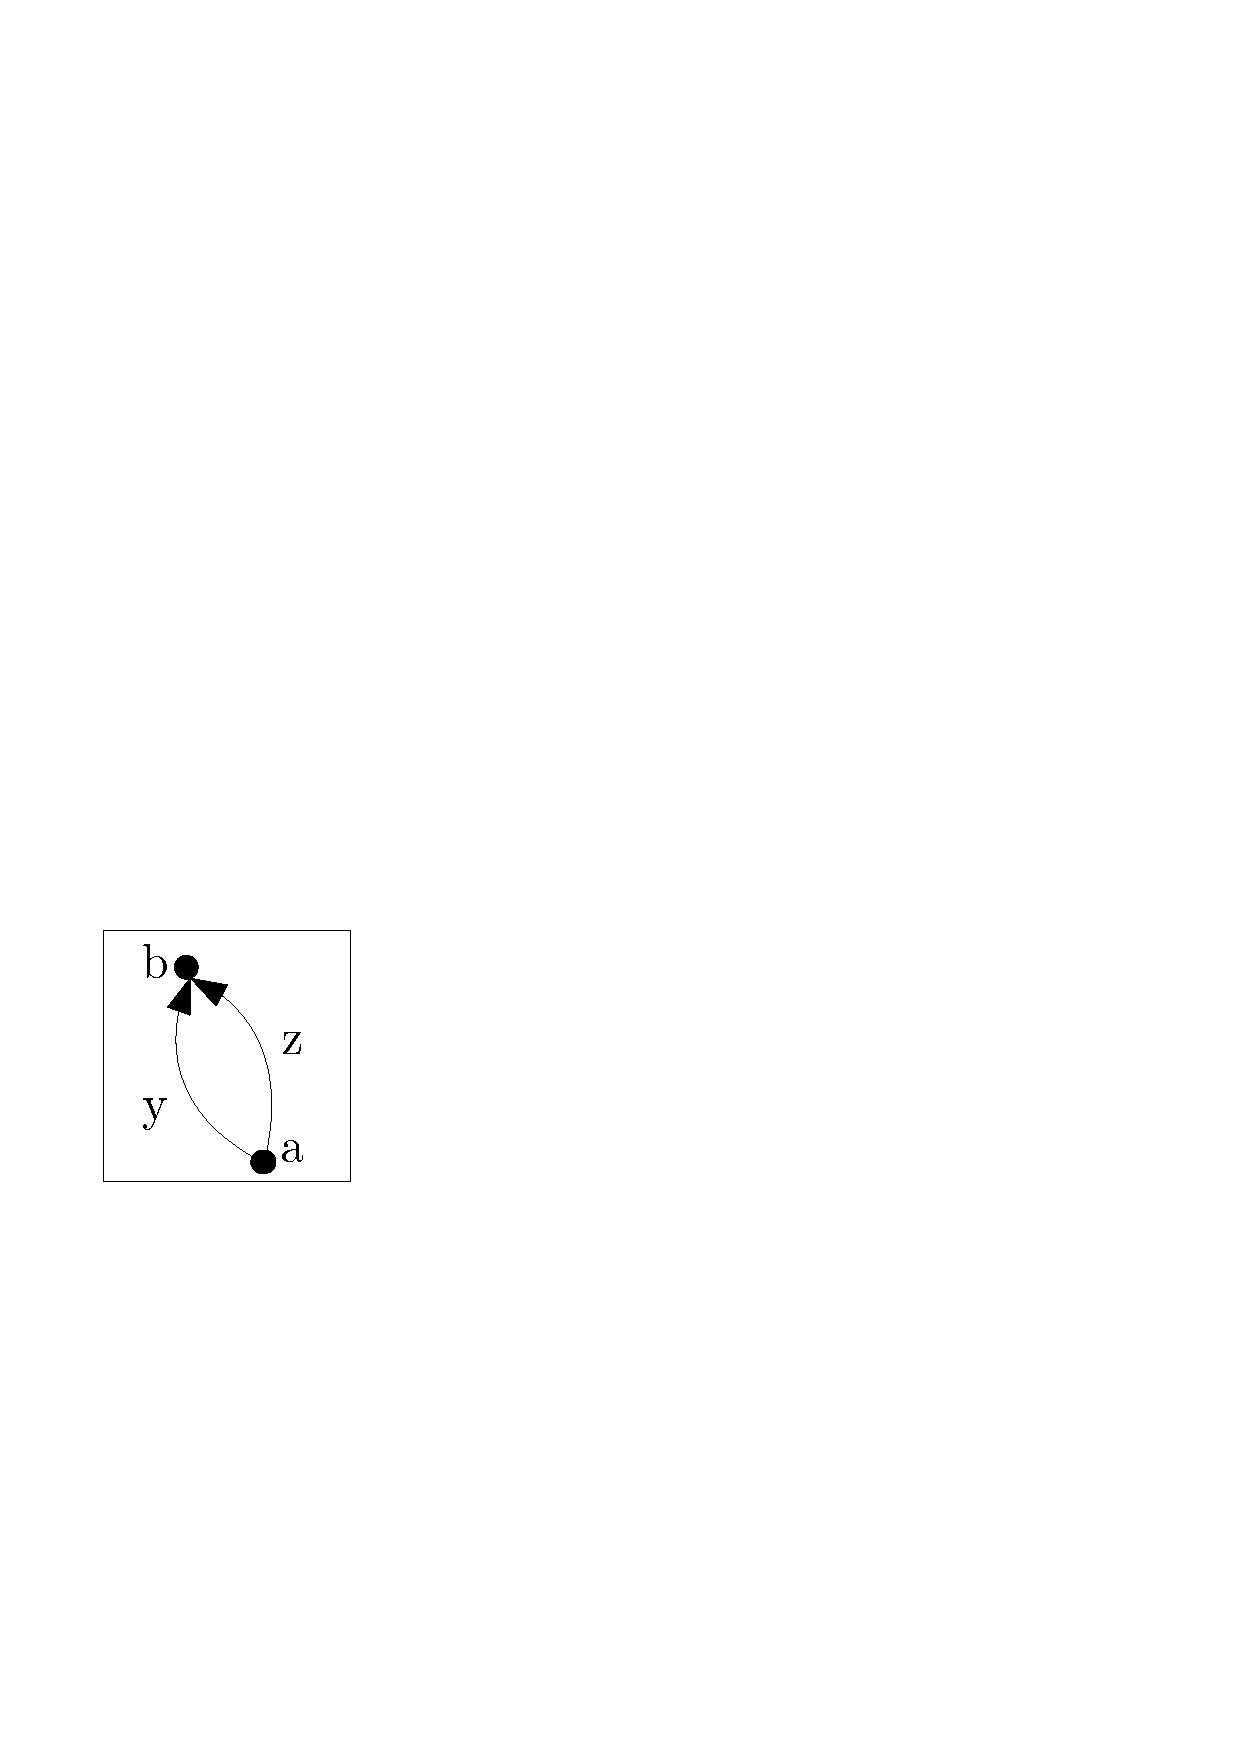
\includegraphics[height=1.25cm]{fig/blatt} \end{array}, \]
apply $p'$ to $H'$ and get the new host graph $H''$, something like this:
\[ 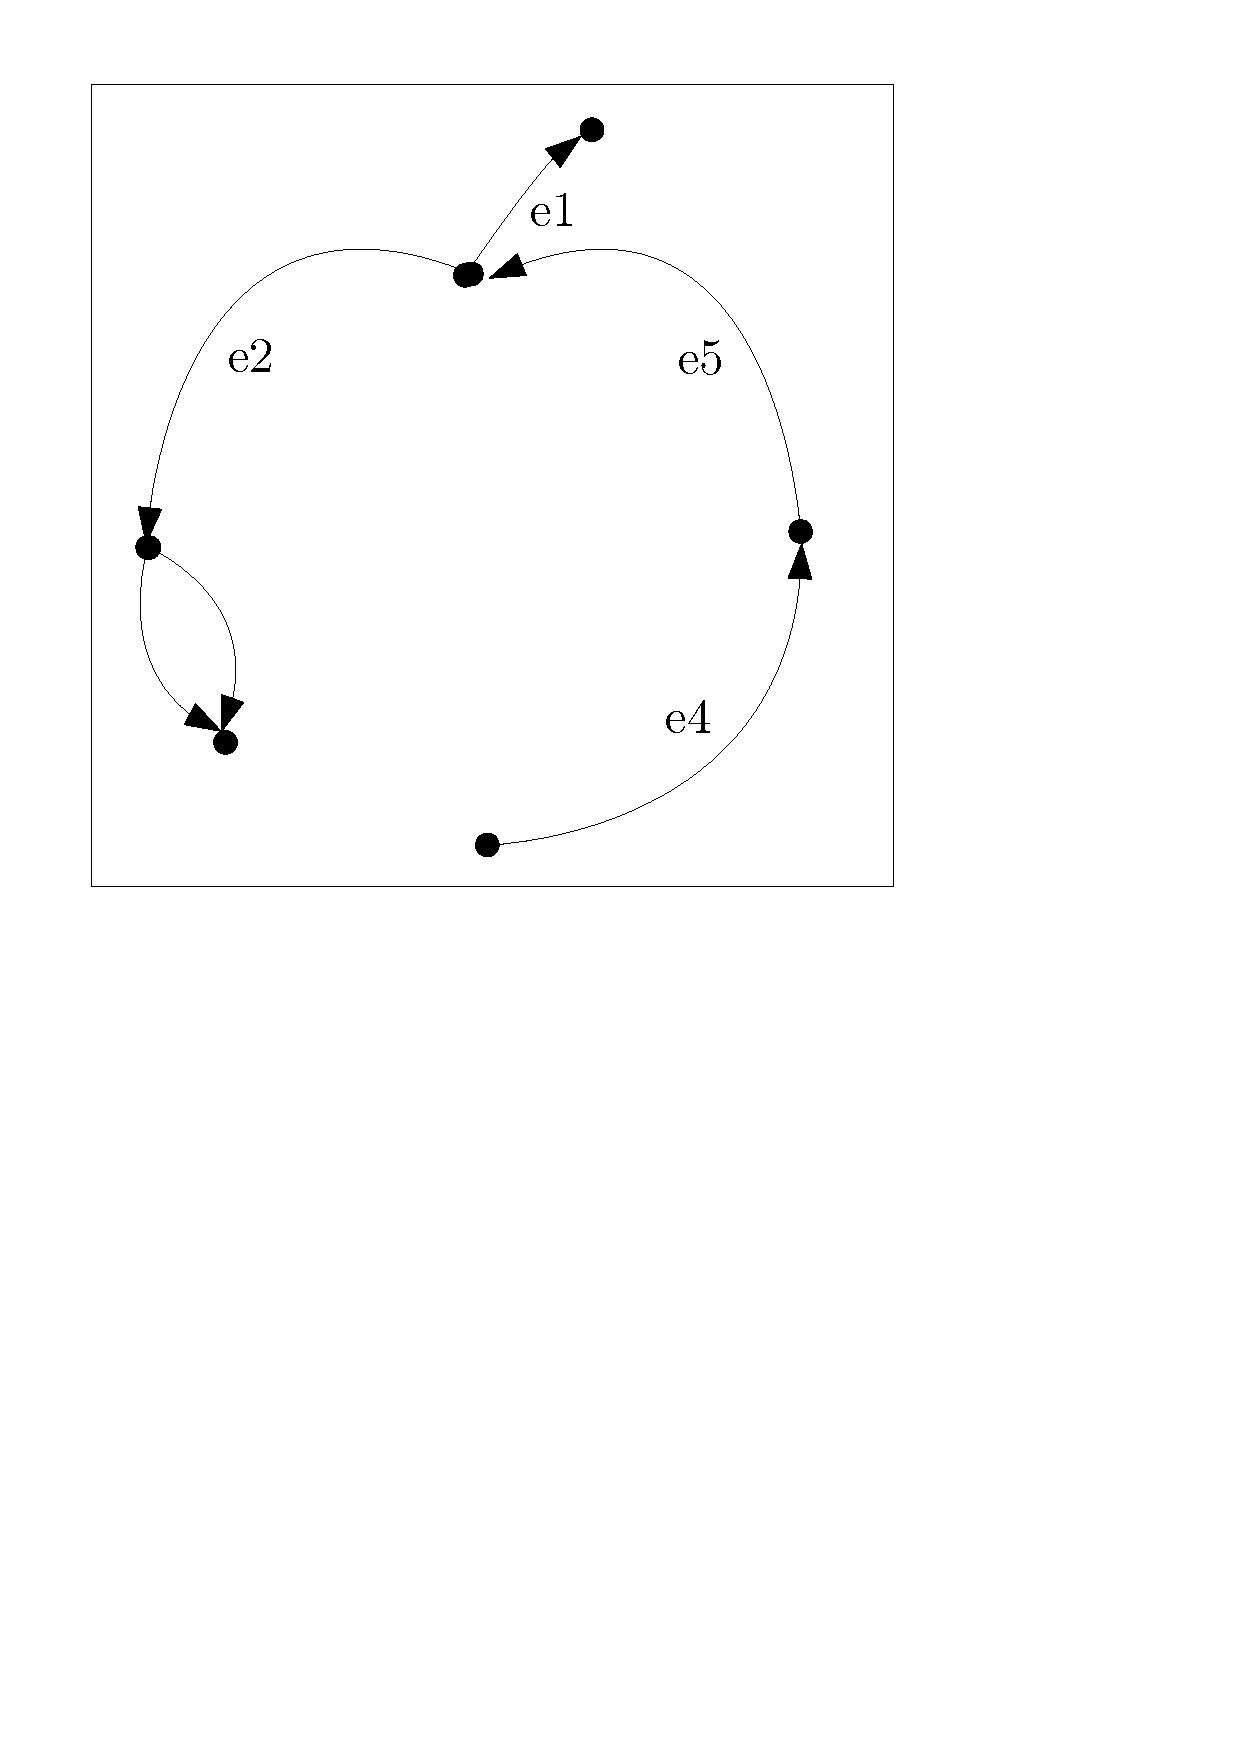
\includegraphics[width=3cm]{fig/wrongapple} \]
What happened? \GrG\ has randomly chosen a match, and $e3$ matches as well as $e1$. A correct solution could make use of edge type information. And this time we'll keep even the stem. So let $H''$ now be
\[ 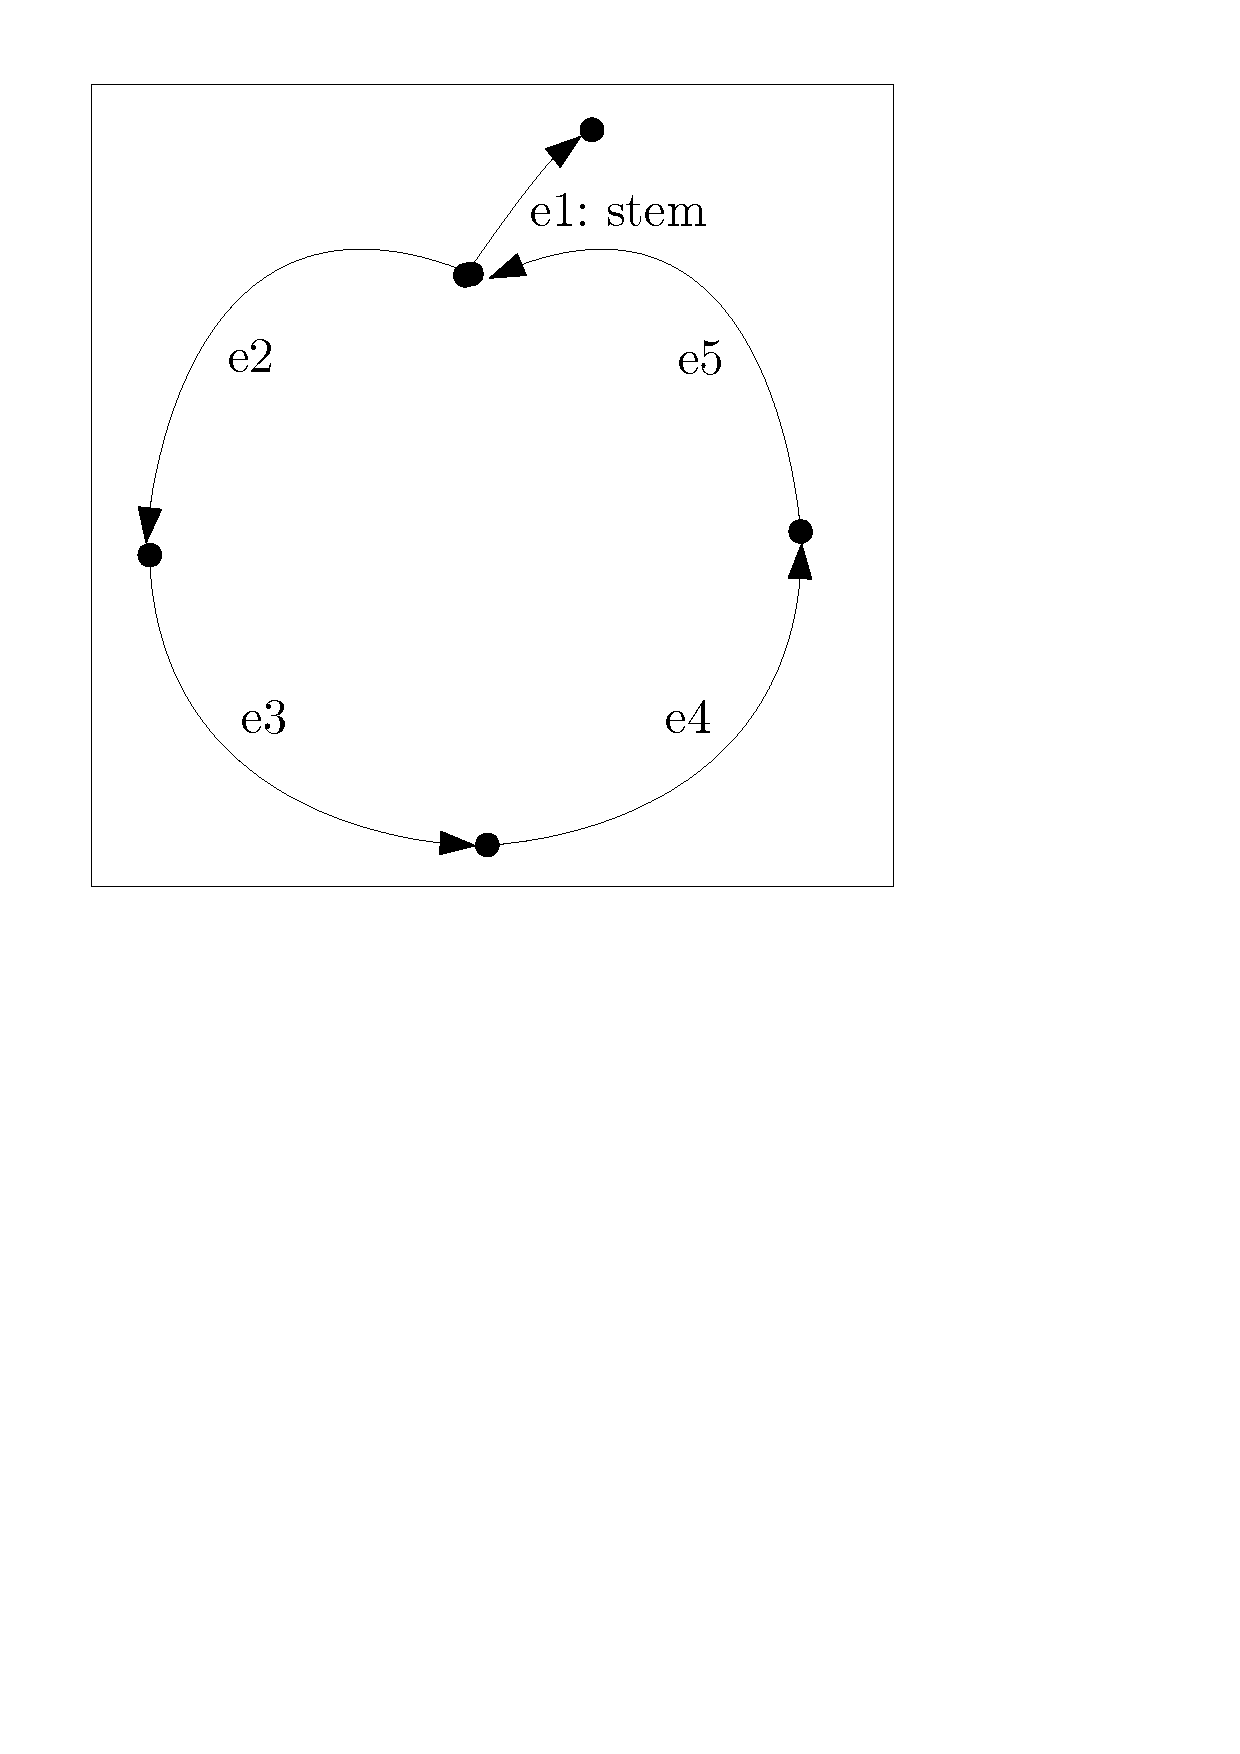
\includegraphics[width=3cm]{fig/typedapple} \]
and
\[ p'':  \begin{array}[c]{c} 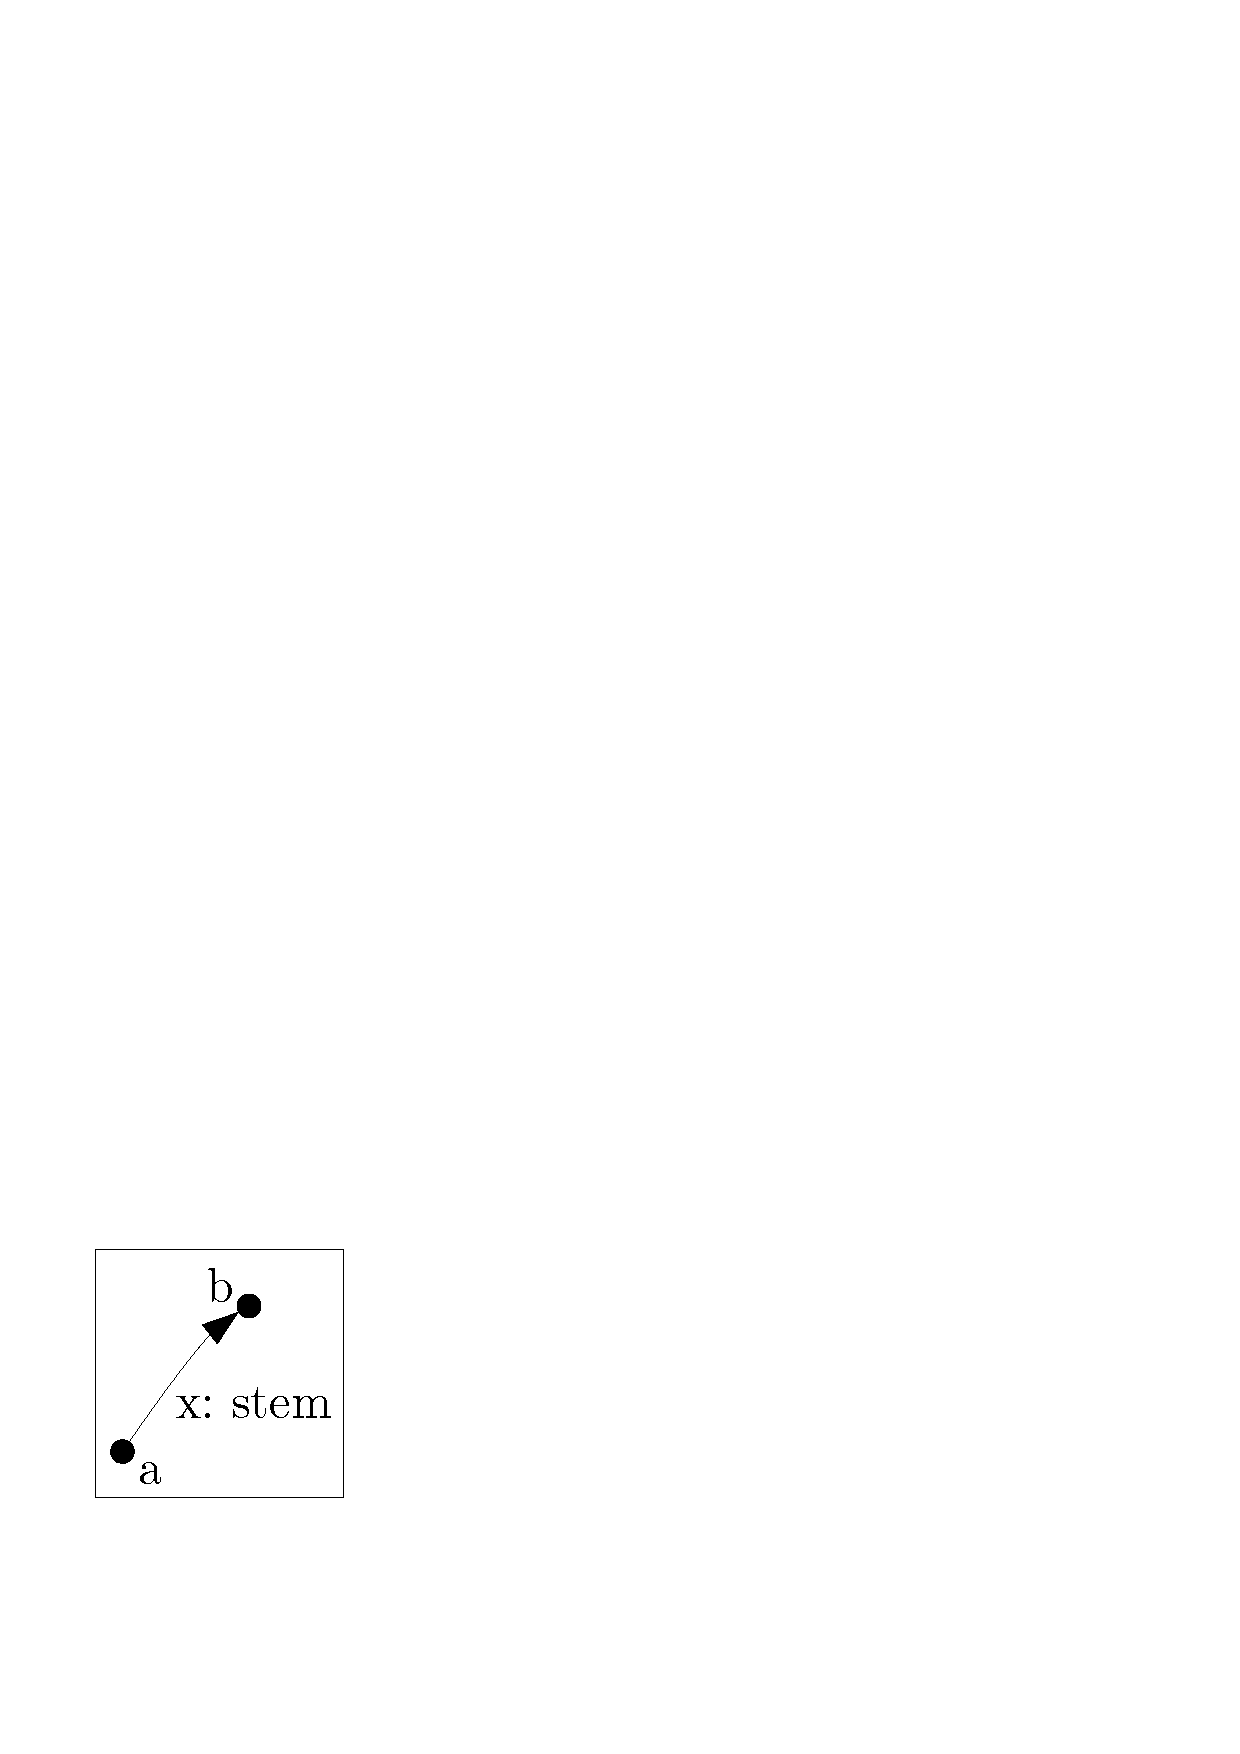
\includegraphics[height=1.25cm]{fig/typedstiel} \end{array} \begin{array}[c]{c} \longrightarrow \end{array} \begin{array}[c]{c} 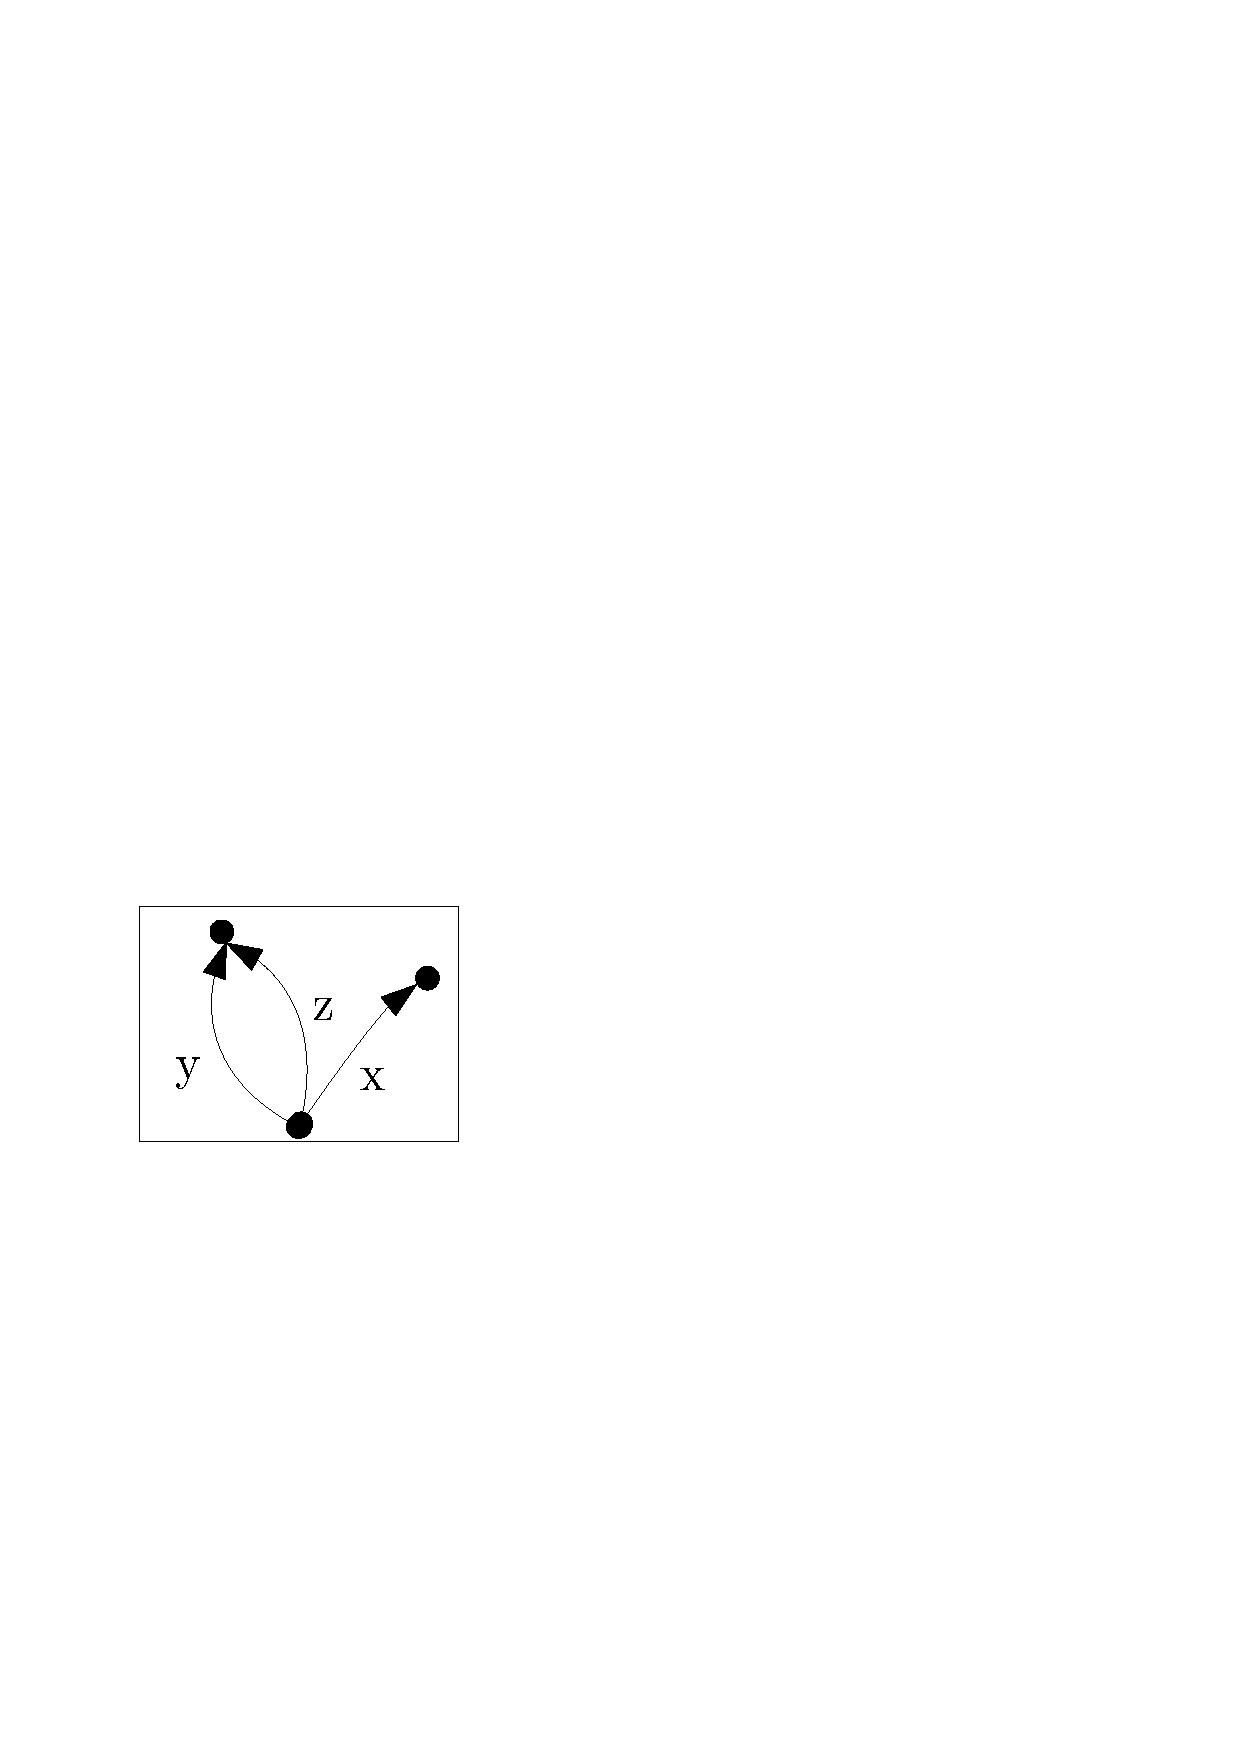
\includegraphics[height=1.25cm]{fig/typedblatt} \end{array}. \]
If we apply $p''$ to $H''$ this leads to
\[ 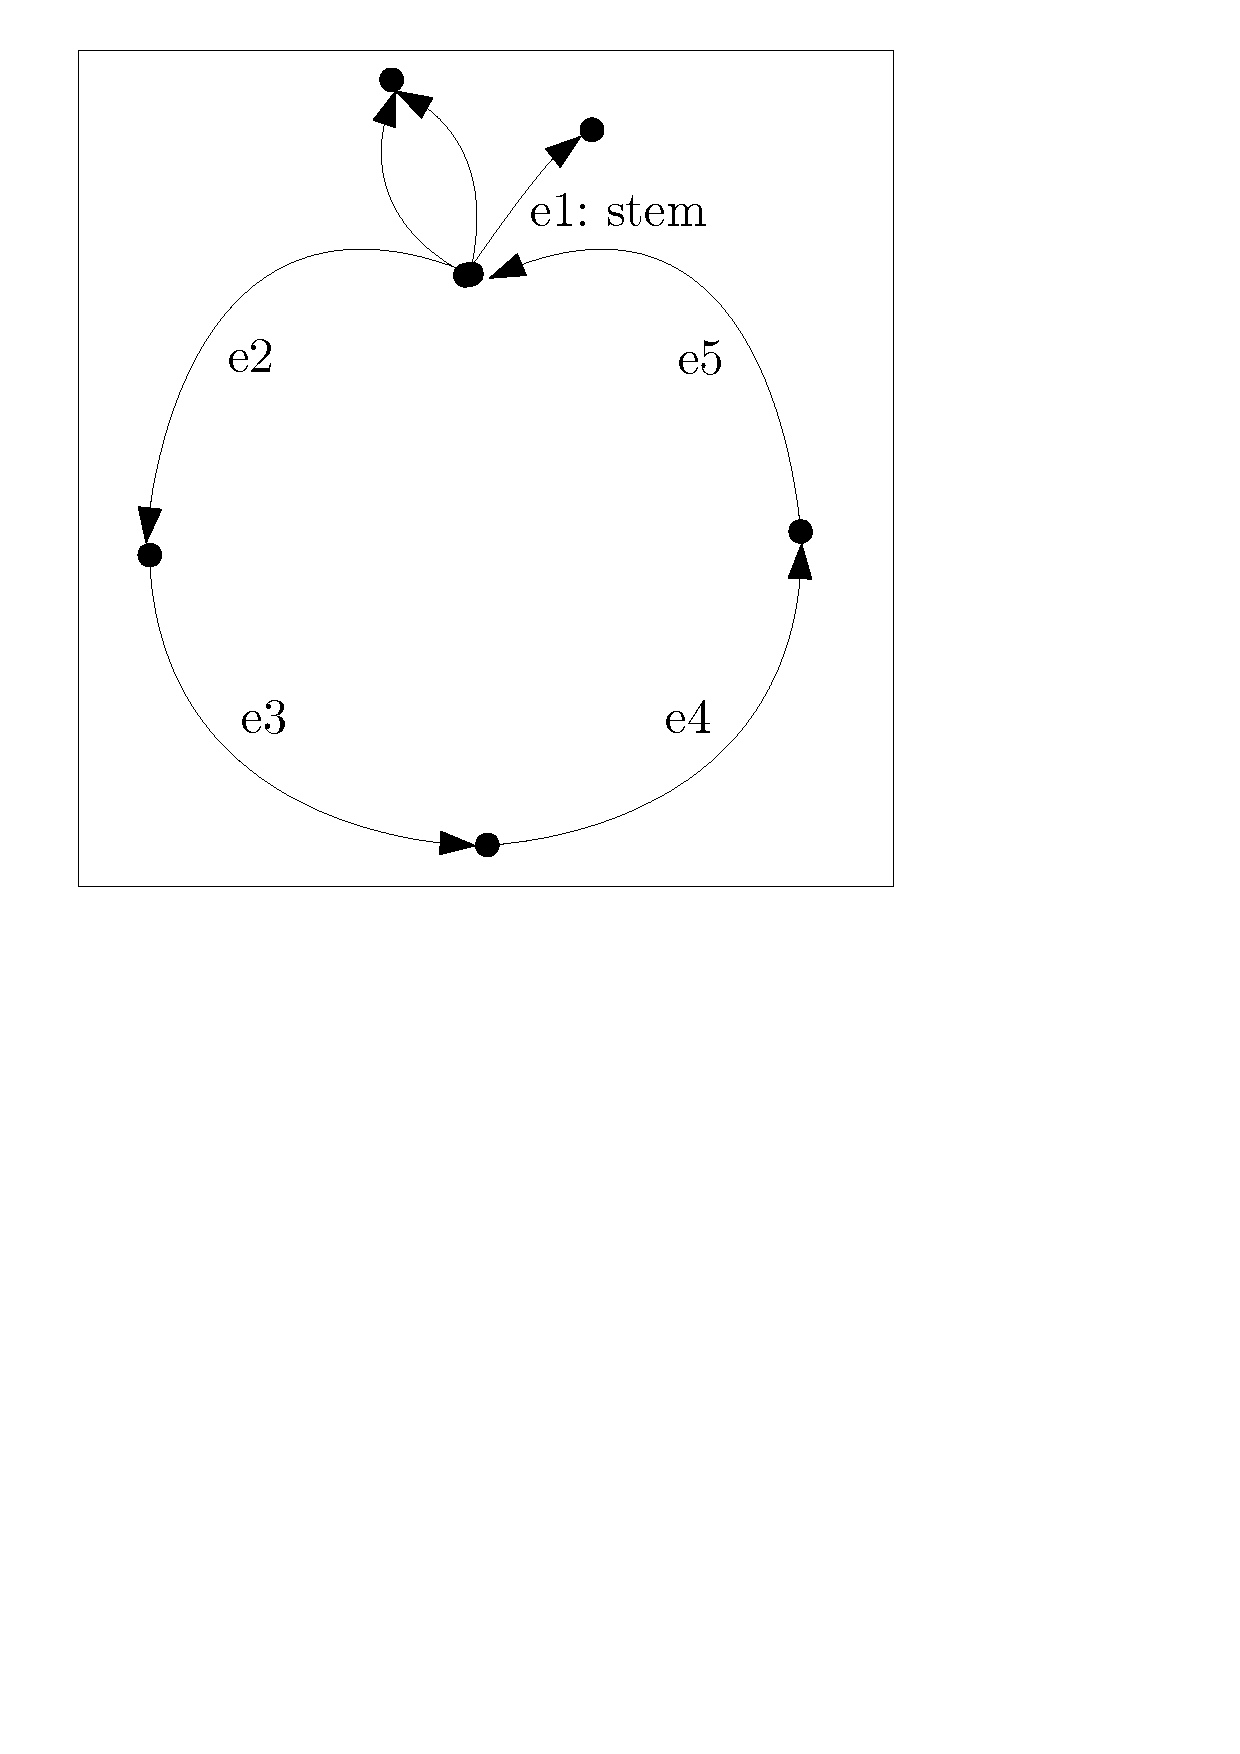
\includegraphics[width=3cm]{fig/rewrittenapple} \]
\emph{Note:} If we had applied $(p')*$ to $H'$ (execute $p'$ consecutively until no match is found) this would not have terminated, because each rewrite had produced one new candidate (one deleted, two added) for matching.    

\section{Components}
Figure \ref{figsys} gives an overview of the \GrG\ system components, whereas table \ref{dirstruc} shows the \GrG\ directory structure.
\begin{figure}[htbp]
  \centering
	\scalebox{0.8}{
  \begin{tikzpicture}
      \begin{scope}[shape=rectangle,minimum size=0.75cm,text width=3cm,text centered]
          \tikzstyle{every node}=[draw]
          \node (spec1)    at (0   ,0)    {Rewrite Rules (*.grg)};
          \node (spec2)    at (0   ,2)    {Graph Model (*.gm)};
          \node (grgen)    at (4   ,1)    {\GrG\ Generator (Java, C\#)};
          \node (rewriter) at (10  ,0)    {Rewrite Rules (C\#)};
          \node (types)    at (10  ,2)    {Graph Model (C\#)};
          \node (data)     at (14  ,1)    {Graph Management (C\#)};
          \node (libgr)    at (12  ,4)    {\LibGr (C\#)};
          \node[fill,color=gray] (app)      at (14.1  ,5.6)  {};
          \node[fill=white] (app)      at (14  ,5.5)  {Applications};
          \node (app2)     at (10  ,5.5)  {\GrShell (C\#)};
      \end{scope}

      \node[draw, minimum width=9cm,minimum height=4cm] (engine) at (12,1) {};
      \node[draw, minimum width=9cm,minimum height=4cm,style=dotted] (ct) at (2,1) {};
      \node[anchor=north east] (engine_lab) at (engine.north east) {Backend (Run Time)};
      \node[anchor=north east] (ct_lab) at (ct.north east) {Frontend (Compile Time)};

      \draw[->,dashed,red,>=triangle 45]     (spec1)   -> (grgen);
      \draw[->,dashed,red,>=triangle 45]     (spec2)   -> (grgen);
      \draw[->,dashed,red,>=triangle 45]     (grgen)   -> (types);
      \draw[->,line width=1pt,>=triangle 45] (grgen)   -> (engine);
      \draw[->,dashed,red,>=triangle 45]     (grgen)   -> (rewriter);
      \draw[->,line width=1pt,>=triangle 45] (app)     -> (libgr);
      \draw[->,line width=1pt,>=triangle 45] (app2)    -> (libgr);
      \draw[->,line width=1pt,>=triangle 45] (libgr)   -> (engine);

      \draw[->,line width=1pt,>=triangle 45] (0,5.125) -- +(2.5,0) node[above, midway] {call};
      \draw[->,dashed,red,>=triangle 45] (0,4.5)  -- +(2.5,0) node[above, midway] {read / generate};
  \end{tikzpicture}
	}
  \caption{\GrG\ system components \cite{kroll}}
  \label{figsys}
\end{figure}

\begin{table}[htbp]
  \begin{tabularx}{\linewidth}{|lX|} \hline
  bin & Contains the .NET assemblies, in particular GrGen.exe (the graph rewriting system generator), LGSPBackend.dll (a \GrG\ backend) and the shell \texttt{GrShell.exe}.  \\ 
  lib & Contains the \GrG\ generated assemblies (*.dll). \\
  specs & Contains the graph rewriting system source documents (*.gm and *.grg). \\ \hline
  \end{tabularx}
  \caption{\GrG\ directory structure}
  \label{dirstruc}
\end{table}

A graph rewriting system is defined by a rule set description file (*.grg) and one or more graph model description files (*.gm).\footnote{System, in this context, is not a CHO-like grammar rewriting system, but rather a set of interacting software components.} It is generated by GrGen.exe and can be used by \GrG\ applications such as \GrShell. Figure \ref{process} shows the generation process.
\begin{figure}[htbp]
  \centering
  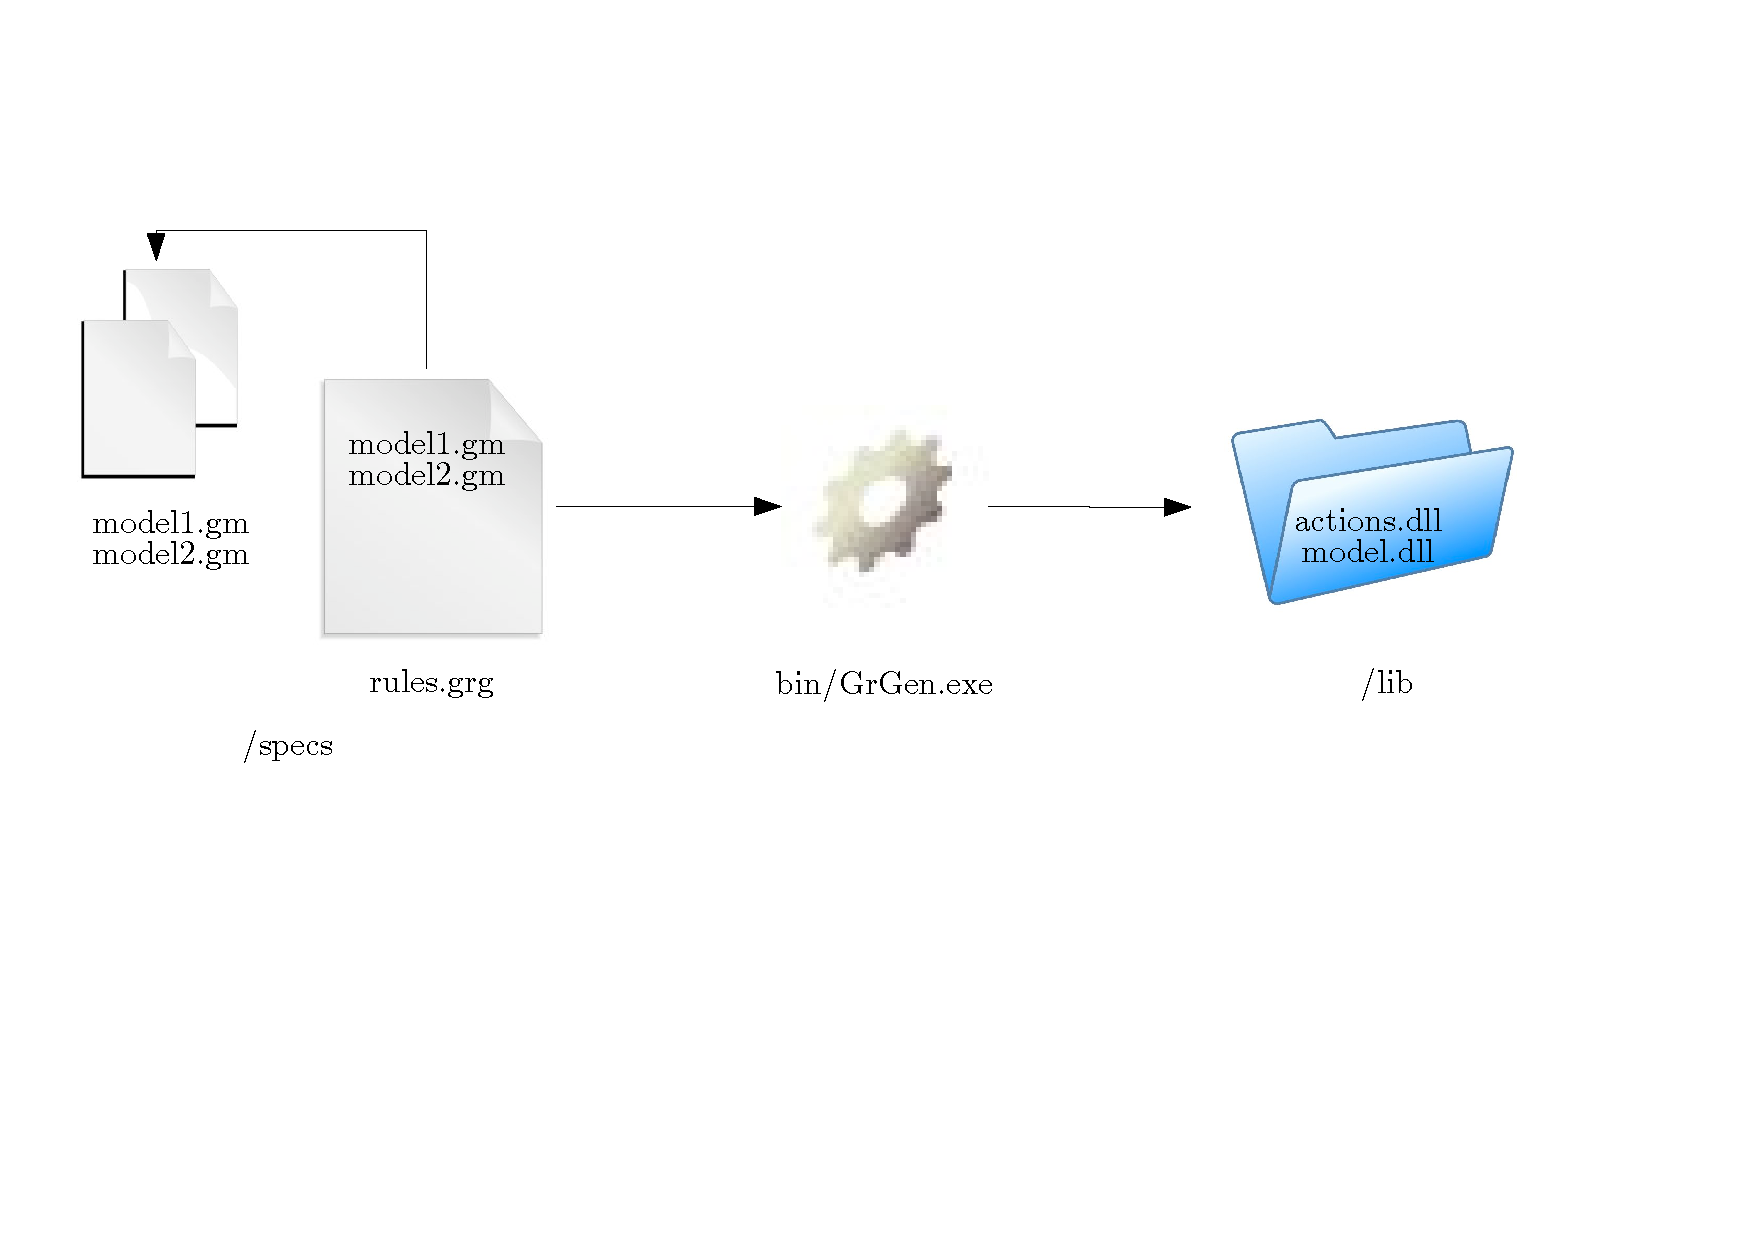
\includegraphics[width=\textwidth]{fig/process}
  \caption{Generating a graph rewriting system}
  \label{process}
\end{figure}

In general you have to distinguish carefully between a graph model (meta level), a host graph, a pattern graph and a rewriting rule. In \GrG\ pattern graphs are implicitly defined by rules, i.e.\ each rule defines its pattern. On the technical side, specification documents for a graph rewriting system can be available as source documents for graph models and rule sets (plain text *.gm and *.grg files) or as their translated .NET modules, either C\# source files or their compiled assemblies (*.dll).

